\documentclass{article}

%%%%%%%%%%%%%%%%%%%%%%%% Importation de paquets %%%%%%%%%%%%%%%%%%%%
\usepackage{polyglossia}
\usepackage{graphics}
\usepackage{fontspec}
\usepackage{fancyhdr}
\usepackage{listings}
\usepackage{graphics}
\usepackage{fancyhdr}
\usepackage{vmargin}
\usepackage{epsfig}   
\usepackage{multicol}
\usepackage{multirow}

%%%%%%%%%%%%%%%%%%%%%%%% Format, langue, marges %%%%%%%%%%%%%%%%%%%%%%%%%%

\setdefaultlanguage{english}
\defaultfontfeatures{Mapping=tex-text,Scale=MatchLowercase}
\setmainfont{Linux Libertine O}
\setpapersize{A4}
\setmarginsrb   
{35mm}  % leftmargin
{20mm}  % topmargin
{35mm}  % rightmargin
{40mm}  % bottommargin
{14pt}  % headheight
{15mm}   % headsep
{20pt}  % footheight
{20mm}  % footskip

%%%%%%%%%%%%%%%%%%%%%%%% En-tete et pied de page %%%%%%%%%%%%%%%%%%%%%%%%%%
\pagestyle{fancy}
\fancyhf{}
\lhead{\scalebox{0.1}[0.1]{
\includegraphics{./Images/enseeiht}}}
\rhead{\scalebox{0.1}[0.1]{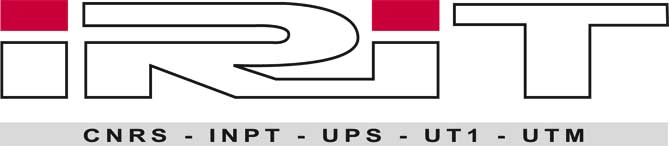
\includegraphics{./Images/irit}}
\lfoot{Three-dimensional modeling and printing}}
\rfoot{\bfseries \thepage}

\begin{document}

\bigskip
\bigskip
\bigskip
\bigskip
\bigskip
\bigskip
\bigskip
\bigskip

\begin{center}
\LARGE{Three-dimensional modeling and printing project :\\Set up documentation : \\}
\bigskip
\bigskip
\Large{from January 23 to March 16, 2012}
\end{center}

\bigskip
\bigskip

\begin{center}
\large{
\textit{Vincent \textsc{Duvert} \\
Antoine \textsc{Lubineau} \\
Caroline \textsc{Naud} \\
James \textsc{Packer} \\
Florian \textsc{Ribon}} \\
\bigskip
INP-ENSEEIHT/IMA 
}
\end{center}

\bigskip
\bigskip

	This report summarizes the context, organization, work and outcomes within the project 3D modeling and printing project suggested by the VORTEX team of IRIT to some of the third-year students in the IMA department of ENSEEIHT.

\bigskip
\bigskip

\begin{figure}[!h]
\begin{center}
\scalebox{0.4}[0.4]{
\includegraphics{./Images/enseeiht}}
\end{center}
\end{figure}

\bigskip

\begin{center}
http://www.enseeiht.fr/fr/index.html \\
2 Rue Charles Camichel \\
31 071 TOULOUSE
\end{center}

\bigskip

\begin{figure}[!h]
\begin{center}
\scalebox{0.4}[0.4]{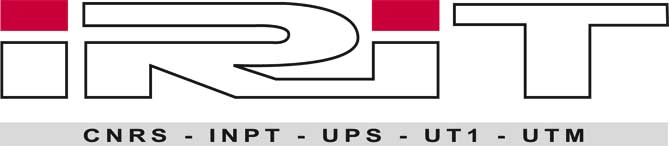
\includegraphics{./Images/irit}}
\end{center}
\end{figure}

\begin{center}
http://www.info@irit.fr\\
Université Paul Sabatier \\
118 Route de Narbonne \\
F-31062 TOULOUSE CEDEX 9
\end{center}

\thispagestyle{empty}

\newpage

\tableofcontents

\newpage

\section{Global architecture of the application}

Here is (in orange) the different software and material you will have to get installed in order to use the complete application. The firmware is integrated in the printer and has not been modified in any way so you won't have to deal with it.

\begin{figure}[!h]
\begin{center}
\scalebox{0.4}[0.4]{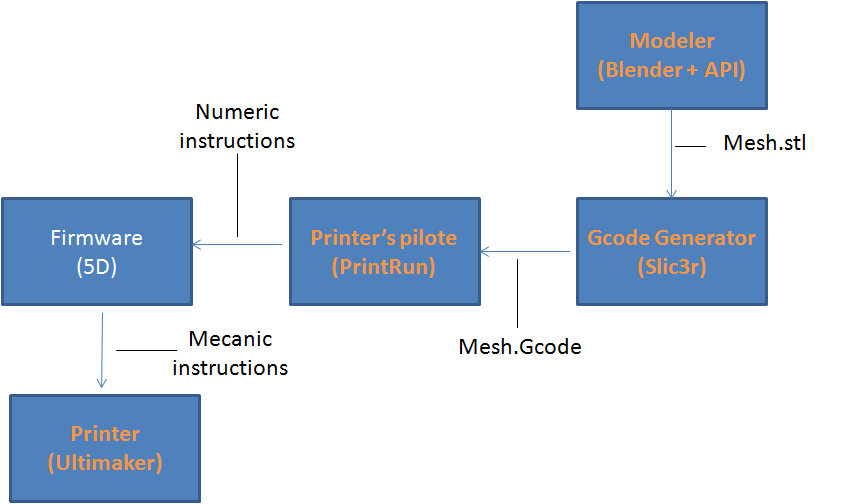
\includegraphics{./Images/ARD1}}
\end{center}
\end{figure}

\newpage

\section{Windows}

\newpage

\section{Ubuntu}

\end{document}
